\scanpage{19}
\[
\left\{\begin{aligned}
\Pi&=(S,A,F;\ R,R',R'';\ E=\mathrm{Rep})\quad\text{icosaèdre combinatoire}\\
\underline a&\quad\text{antipodisme}\qquad a\in G=\mathrm{Aut}(\Pi)
\end{aligned}\right.
\]
\margin{opère sans pts fixes sur $S,A,F$ (et a fortiori sur $R,R',R'',E$)}
\[
\begin{aligned}
\bar A&=A/\underline a\qquad\text{ens des quinze}\\
&\hspace{3em}\text{``directions d'arêtes''}\\
a&\longmapsto\bar a\quad\text{appl. canonique }A\longrightarrow\bar A
\end{aligned}
\]
\margin{(terminologie : arêtes \uline{parallèles})}
On va définir une permutation canonique
\[
\rho:\bar A\longrightarrow\bar A
\]
Pour ceci, pour $a\in A$, soit $s\in S$ incident à $a$. Considérons les \deleted{deux} arêtes \inserted{$\{s,u\},\{s,v\}$} \deleted{dans} $\unsure{\mathscr P|P|\Phi}_{\geq s}$ adjacentes à $a=\{s,t\}$, considérons les deux autres $\{s,\deleted{\unsure{s_u}}\pi_{s,u}\},\{s,\deleted{\unsure{s_v}}\pi_{s,v}\}$ restantes parmi les cinq de $\mathscr P_{\geq s}$, alors $\{s_u,s_v\}$ est une arête de $\Pi$. [On peut dire que les cinq sommets adjacents à $s$ forment un pentagone ayant comme sommet distingué le deuxième sommet $t$ de $a$, et on prend le côté de ce pentagone \uline{opposé} à ce sommet $t$.]

\figure{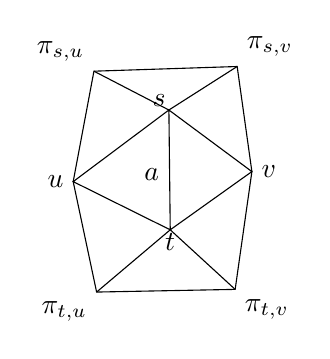
\begin{tikzpicture}[x=.85cm,y=.85cm]
\coordinate (lu) at (-1.12,1.65); \coordinate (ru) at (1.02,1.72);
\coordinate (u) at (-1.43,0); \coordinate (v) at (1.24,.15);
\coordinate (s) at (0,1.07); \coordinate (t) at (.02,-.72);
\coordinate (ld) at (-1.08,-1.65); \coordinate (rd) at (.99,-1.61);
\draw (lu)--(ru)--(v)--(rd)--(ld)--(u)--cycle;
\draw (lu)--(s)--(ru) (s)--(u)--(t)--(v)--(s)--(t) (ld)--(t)--(rd);
\node[above left] at (lu) {$\pi_{s,u}$}; \node[above right] at (ru) {$\pi_{s,v}$};
\node[left] at (u) {$u$}; \node[right] at (v) {$v$};
\node[above left,inner sep=1pt] at (s) {$s$}; \node[below,inner sep=1pt] at (t) {$t$};
\node[left] at (0,.1) {$a$}; \node[below left] at (ld) {$\pi_{t,u}$};
\node[below right] at (rd) {$\pi_{t,v}$};
\end{tikzpicture}}

Si on avait pris l'autre sommet $t$, on aurait trouvé l'arête $\{\deleted{\unsure{t_u}}\pi_{t,u},\deleted{\unsure{t_v}}\pi_{t,v}\}$ antipodique de $\{s_u,s_v\}$, d'où un unique élément $\rho_0(a)\in\bar A$. On trouve \inserted{ainsi} une application canonique
\[
 A\longrightarrow\bar A
\]
qui commute aux autom de $\Pi$, et en particulier à $\underline a$. Comme $\underline a$ opère trivialement sur $\bar A$, \deleted{\unsure{$\exists$}} $\rho_0$ se factorise en
\[
\bar A\longrightarrow\bar A
\]
On trouve
\[
\rho^2(\bar a)=\overline{\{u,v'\}}=\overline{\{v,u'\}}
\]
% archive sheet number: 18
